%==============================================================================
%  MASTER'S THESIS DEFENCE  --  ~25 minutes, 17 content slides
%  Spine: classic engineering arc (B) + battery-cheating twist (A)
%  Audience: some RL knowledge, NO automotive  ->  explain powertrain/NOx lightly
%  Compile: pdflatex defense.tex  (x3 for refs)  -- run from TFM/defense/
%==============================================================================
\documentclass[aspectratio=169,11pt]{beamer}

\usetheme{Madrid}
\usecolortheme{whale}

% --- clean, modern-ish colour palette -----------------------------------
\definecolor{tugreen}{RGB}{0,110,114}     % primary teal
\definecolor{tudark}{RGB}{30,40,55}       % titles
\definecolor{tuaccent}{RGB}{210,90,40}    % warnings / honesty accents
\setbeamercolor{structure}{fg=tugreen}
\setbeamercolor{frametitle}{bg=tugreen,fg=white}
\setbeamercolor{title}{fg=white}
\setbeamercolor{alerted text}{fg=tuaccent}
\setbeamertemplate{navigation symbols}{}
\setbeamertemplate{caption}{\raggedright\insertcaption\par}
\setbeamerfont{frametitle}{size=\large}
\setbeamertemplate{itemize items}[circle]

\usepackage[utf8]{inputenc}
\usepackage{booktabs}
\usepackage{graphicx}
\usepackage{amsmath}
\usepackage{xcolor}
\graphicspath{{../imgs/}}

% short footline: author -- short title -- frame number
\setbeamertemplate{footline}{%
  \leavevmode%
  \hbox{%
    \begin{beamercolorbox}[wd=.30\paperwidth,ht=2.25ex,dp=1ex,center]{author in head/foot}%
      \usebeamerfont{author in head/foot}N. Long Schiefelbein%
    \end{beamercolorbox}%
    \begin{beamercolorbox}[wd=.50\paperwidth,ht=2.25ex,dp=1ex,center]{title in head/foot}%
      \usebeamerfont{title in head/foot}RL-Based NO\textsubscript{x} Control for a Hybrid Diesel Vehicle%
    \end{beamercolorbox}%
    \begin{beamercolorbox}[wd=.20\paperwidth,ht=2.25ex,dp=1ex,right]{date in head/foot}%
      \usebeamerfont{date in head/foot}\insertframenumber/\inserttotalframenumber\hspace*{2ex}%
    \end{beamercolorbox}}%
  \vskip0pt%
}

% helper macros
\newcommand{\NOx}{NO\textsubscript{x}}
\newcommand{\keyword}[1]{\textcolor{tugreen}{\textbf{#1}}}
\newcommand{\honest}[1]{\textcolor{tuaccent}{\textbf{#1}}}

%------------------------------------------------------------------------------
\title[RL NOx Control]{Reinforcement-Learning-Based Control for\\ \NOx{} Emission Reduction in a Hybrid Diesel Vehicle}
\author[N. Long Schiefelbein]{Niklas Long Schiefelbein}
\institute[UPC]{Master's Thesis Defence \\ Supervisor: Cecilio Angulo Bahón \\[0.4em] IDEAI -- Universitat Politècnica de Catalunya \\ within the LDCI2027 / CORNET project}
\date{2026}

%==============================================================================
\begin{document}

% --- 1. TITLE  (0:30) ---------------------------------------------------------
{\setbeamertemplate{footline}{}
\begin{frame}[plain]
  \titlepage
\end{frame}}

% --- roadmap ------------------------------------------------------------------
\begin{frame}{Roadmap}
  \tableofcontents
\end{frame}

%==============================================================================
\section{Motivation \& Problem}
%==============================================================================

% --- 2. MOTIVATION  (2:00) ----------------------------------------------------
\begin{frame}{Why this matters: clean hybrid powertrains}
  \begin{columns}[T]
    \begin{column}{0.56\textwidth}
      \begin{itemize}
        \item Transport $\approx$ \keyword{one third} of EU greenhouse-gas emissions.
        \item Combustion cars still $\approx$ 31\,\% of new sales $\Rightarrow$ improving them still matters.
        \item \keyword{Hybrid Electric Vehicles (HEV)} = bridge: combustion range + electric efficiency.
        \item Our target pollutant: \keyword{\NOx{}} (nitrogen oxides) -- a health hazard, capped by \keyword{Euro 6 at 80\,mg/km}.
      \end{itemize}
      \vspace{0.5em}
      \footnotesize Goal of this work: make an HEV emit \emph{less} \NOx{} without breaking anything else.
    \end{column}
    \begin{column}{0.44\textwidth}
      \centering
      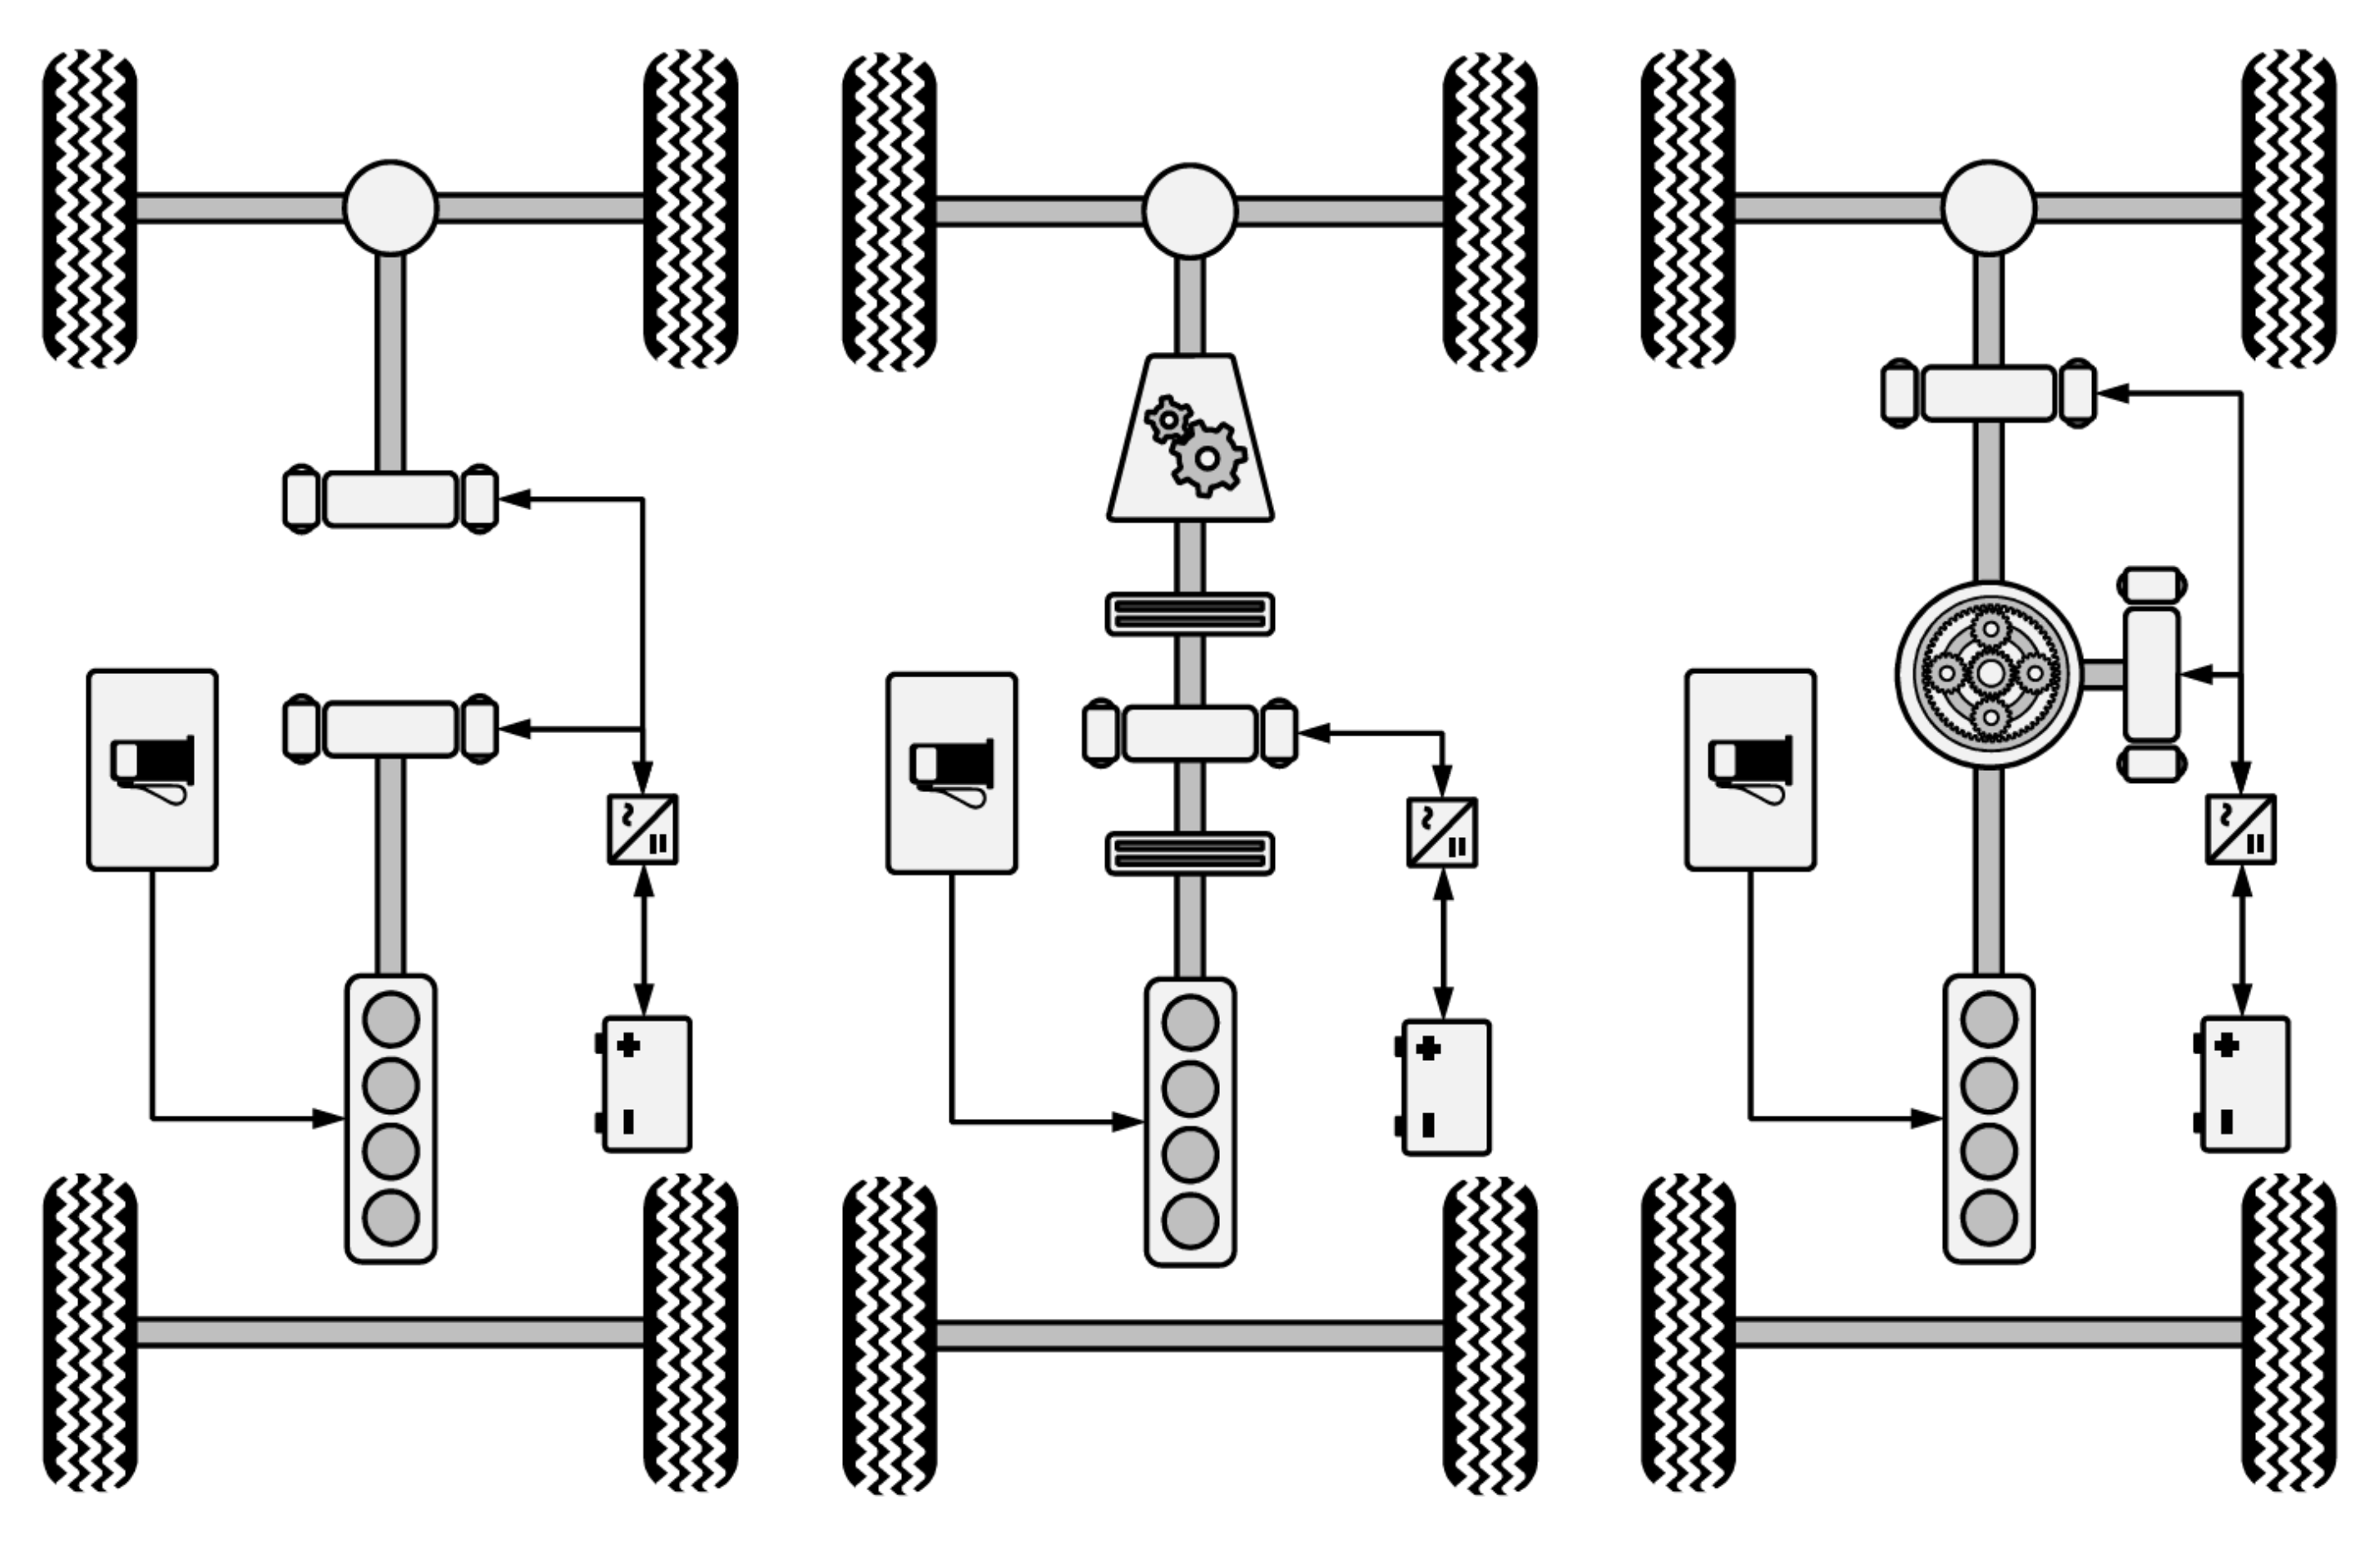
\includegraphics[width=\linewidth,height=0.7\textheight,keepaspectratio]{powertrains.png}
      \par\tiny Powertrain architectures.
    \end{column}
  \end{columns}
\end{frame}

% --- 3. THE CONTROL PROBLEM  (2:30) -------------------------------------------
\begin{frame}{The control problem: four goals fighting at once}
  An HEV controller must \keyword{simultaneously}:
  \begin{columns}[T]
    \begin{column}{0.5\textwidth}
      \begin{enumerate}
        \item follow the \keyword{driver's speed}
        \item cut \keyword{\NOx{}} emissions
        \item keep the \keyword{battery charged} (charge-sustaining)
        \item decide in \keyword{$<$ 1\,ms} (real time)
      \end{enumerate}
    \end{column}
    \begin{column}{0.5\textwidth}
      \footnotesize Every classical method breaks somewhere:
      \begin{itemize}\footnotesize
        \item \textbf{Dynamic Programming} -- optimal, but needs the \emph{whole future} + too slow.
        \item \textbf{Rule-based} -- reliable, but hand-tuned per vehicle.
        \item \textbf{MPC / ECMS} -- need forecasts / constant retuning.
      \end{itemize}
    \end{column}
  \end{columns}
  \vspace{0.6em}
  \centering
  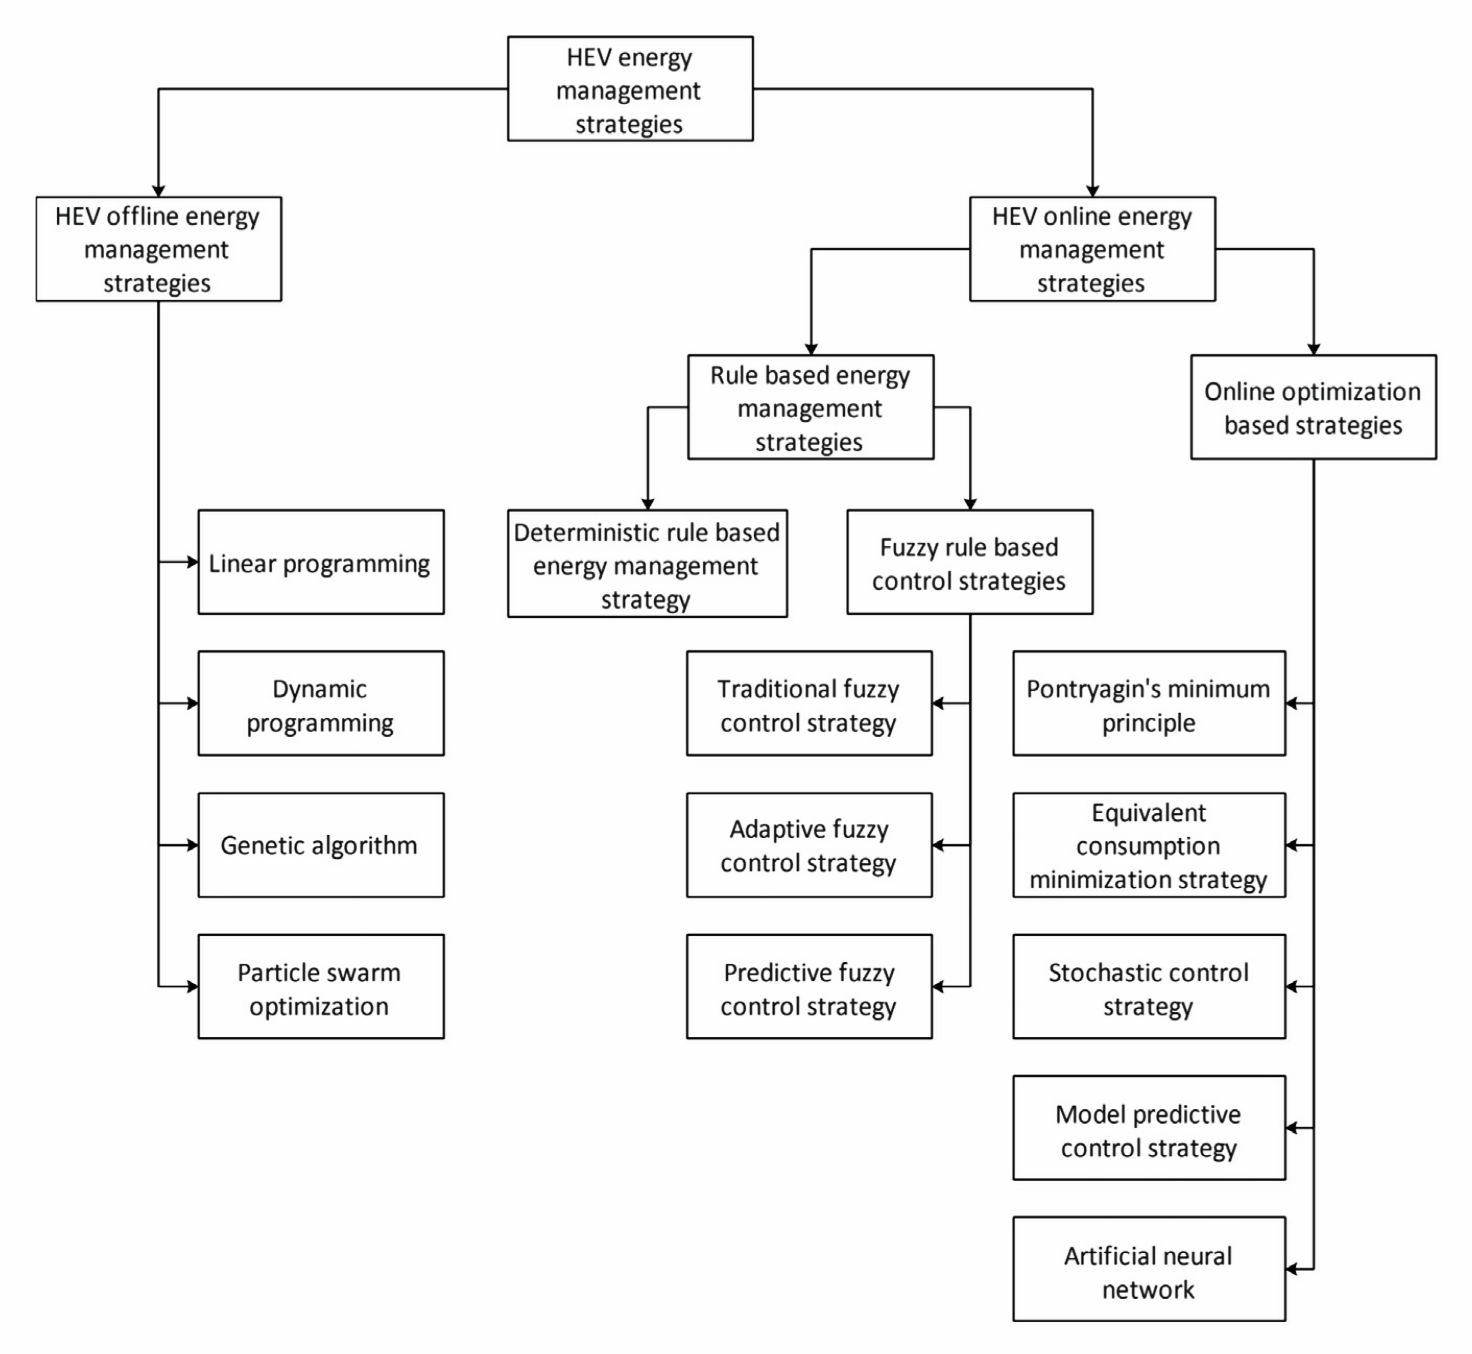
\includegraphics[width=\textwidth,height=0.40\textheight,keepaspectratio]{topology_control_strategies.png}
\end{frame}

% --- 4. WHY RL + PROJECT CONTEXT  (2:00) --------------------------------------
\begin{frame}{Why Reinforcement Learning -- and where this thesis sits}
  \begin{columns}[T]
    \begin{column}{0.55\textwidth}
      \keyword{RL} promises to handle all four jointly:
      \begin{itemize}
        \item learns \keyword{offline}, runs \keyword{instantly} (one forward pass)
        \item \keyword{no hand-written rules} -- learns from interaction
        \item naturally \keyword{multi-objective} via the reward
      \end{itemize}
      \vspace{0.6em}
      \textbf{Project context (LDCI2027):}
      \footnotesize
      \begin{itemize}\footnotesize
        \item TU Berlin = engine test bench, IFS = plant models, \keyword{UPC = control (this work)}.
      \end{itemize}
    \end{column}
    \begin{column}{0.45\textwidth}
      \footnotesize \textbf{Honest starting point:}\\[0.3em]
      Prior project work could not even \emph{stabilise} the speed.\\[0.4em]
      This thesis \keyword{steps back} to get something that works:
      \begin{itemize}\footnotesize
        \item non-recurrent agents
        \item approximate the problem as an \keyword{MDP}
        \item track a \keyword{full trajectory}, not one fixed speed
      \end{itemize}
    \end{column}
  \end{columns}
\end{frame}

%==============================================================================
\section{Approach}
%==============================================================================

% --- 5. SURROGATE ENVIRONMENT  (1:30) -----------------------------------------
\begin{frame}{Training environment: a fast LSTM surrogate}
  \begin{columns}[T]
    \begin{column}{0.46\textwidth}
      \begin{itemize}
        \item Physical engine simulation is \keyword{too slow} for millions of RL steps.
        \item Replace it with two cascaded \keyword{LSTM} surrogate models:
        \begin{itemize}
          \item \textbf{ICE} surrogate $\to$ torque + \NOx{}
          \item \textbf{drivetrain} surrogate $\to$ speed + battery state
        \end{itemize}
        \item Closed loop: agent acts $\to$ surrogate predicts $\to$ reward $\to$ repeat.
      \end{itemize}
    \end{column}
    \begin{column}{0.54\textwidth}
      \centering
      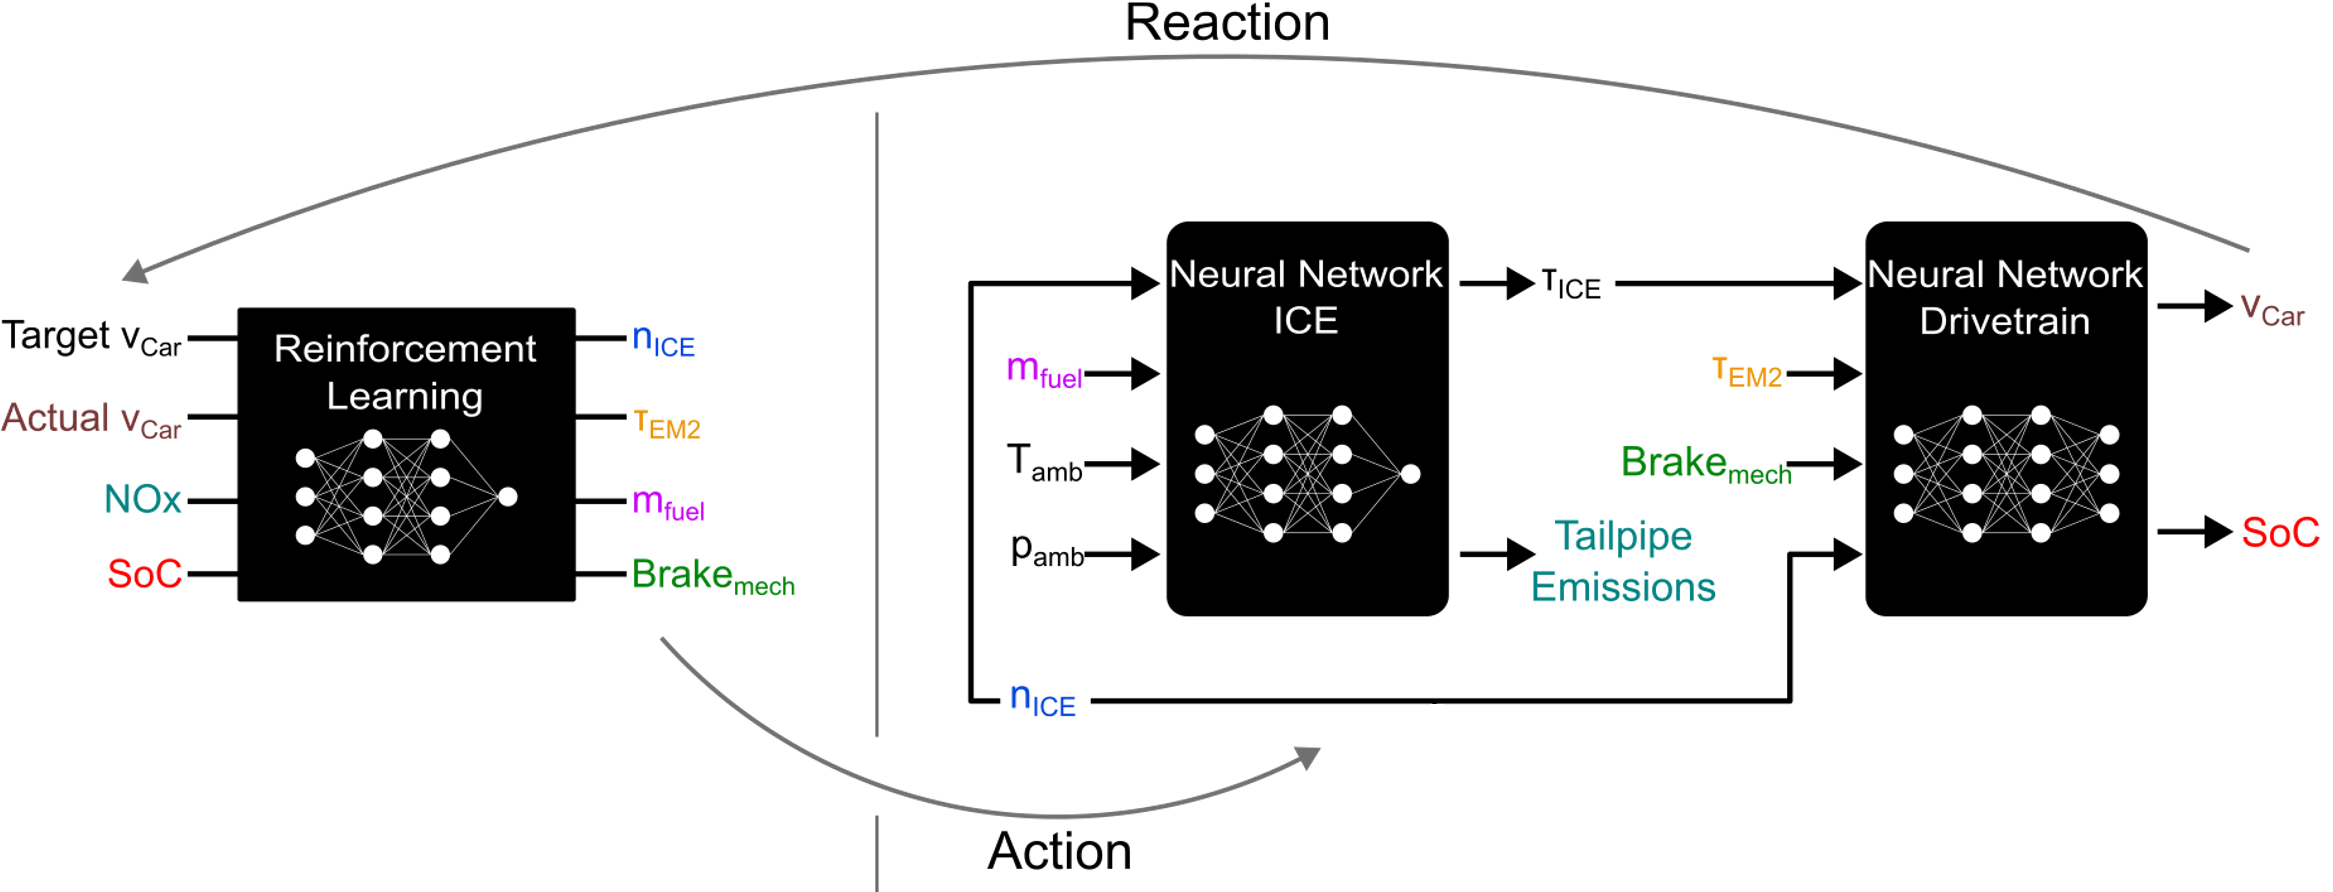
\includegraphics[width=\linewidth,height=0.72\textheight,keepaspectratio]{control_flow.png}
    \end{column}
  \end{columns}
\end{frame}

% --- 6. RL FORMULATION  (2:00) ------------------------------------------------
\begin{frame}{What the agent sees, does, and is rewarded for}
  \begin{columns}[T]
    \begin{column}{0.33\textwidth}
      \textbf{Observes} \footnotesize(measurable only)
      \begin{itemize}\footnotesize
        \item speed + tracking error
        \item battery state (SOC)
        \item engine state, fuel, \NOx{}
        \item 1 thermal proxy (SCR temp)
        \item last actions
      \end{itemize}
    \end{column}
    \begin{column}{0.33\textwidth}
      \textbf{Controls}
      \begin{itemize}\footnotesize
        \item engine on/off + rpm
        \item electric-motor torque
        \item fuel injected
        \item mechanical brake
      \end{itemize}
    \end{column}
    \begin{column}{0.33\textwidth}
      \textbf{Reward}
      \begin{itemize}\footnotesize
        \item core: \keyword{speed tracking} (peak at zero error)
        \item penalties: \NOx{}, SOC drift
        \item small shaping: braking, engine flicker
      \end{itemize}
    \end{column}
  \end{columns}
  \vspace{0.8em}
  \begin{block}{Key principle}
    The reward is only a \keyword{proxy}. Agents are selected on the \keyword{true measured objective} (speed RMSE), \emph{not} on accumulated reward.
  \end{block}
\end{frame}

% --- 7. CURRICULUM  (1:30) ----------------------------------------------------
\begin{frame}{The core method idea: a two-phase curriculum}
  Don't learn everything at once -- learn to \emph{walk} before you optimise.
  \begin{columns}[T]
    \begin{column}{0.5\textwidth}
      \begin{block}{Phase 1 -- Feasibility}
        Reward = \keyword{speed tracking only}.\\
        Question: can RL drive the car at all? What side-effects appear?
      \end{block}
    \end{column}
    \begin{column}{0.5\textwidth}
      \begin{block}{Phase 2 -- Multi-objective}
        \keyword{Warm-start} from Phase 1, then \keyword{add \NOx{} + SOC} penalties.\\
        Question: can we get clean + charge-sustaining \emph{without losing tracking}?
      \end{block}
    \end{column}
  \end{columns}
  \vspace{0.4em}
  \centering
  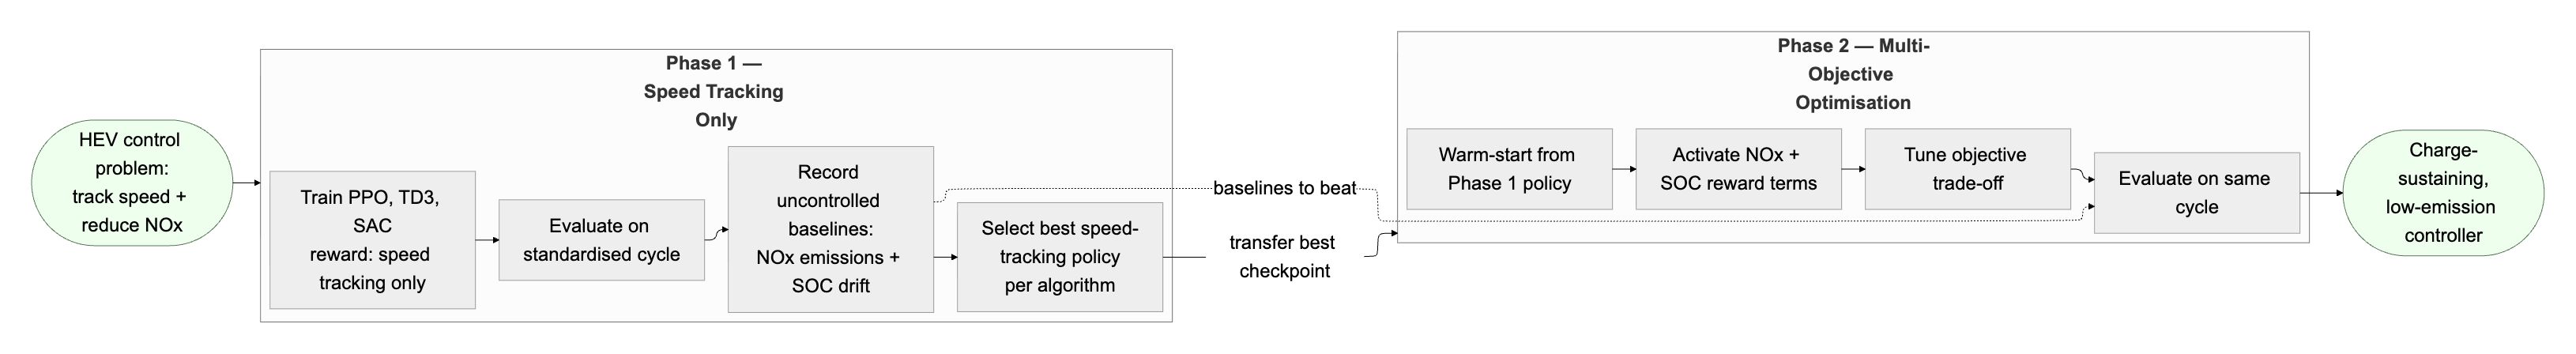
\includegraphics[width=\textwidth,height=0.40\textheight,keepaspectratio]{overall_methodology.png}
\end{frame}

% --- 8. ALGORITHMS + EVAL  (1:30) ---------------------------------------------
\begin{frame}{Algorithms and evaluation protocol}
  \begin{columns}[T]
    \begin{column}{0.5\textwidth}
      \textbf{Three actor--critic algorithms}
      \begin{itemize}
        \item \keyword{PPO} -- simple, on-policy baseline (sanity check)
        \item \keyword{SAC} -- off-policy, sample-efficient
        \item \keyword{TD3} -- off-policy, used in related HEV work
      \end{itemize}
      \footnotesize Hyperparameters chosen with \keyword{Optuna}; each config re-trained over \keyword{10 seeds}.
    \end{column}
    \begin{column}{0.5\textwidth}
      \textbf{Evaluation}
      \begin{itemize}\footnotesize
        \item deterministic \keyword{staircase} speed cycle
        \item primary metric: speed \keyword{RMSE}
        \item diagnostics: cumulative \NOx{}, fuel, $\Delta$SOC
        \item report mean\,$\pm$\,std over 10 seeds
      \end{itemize}
      \centering
      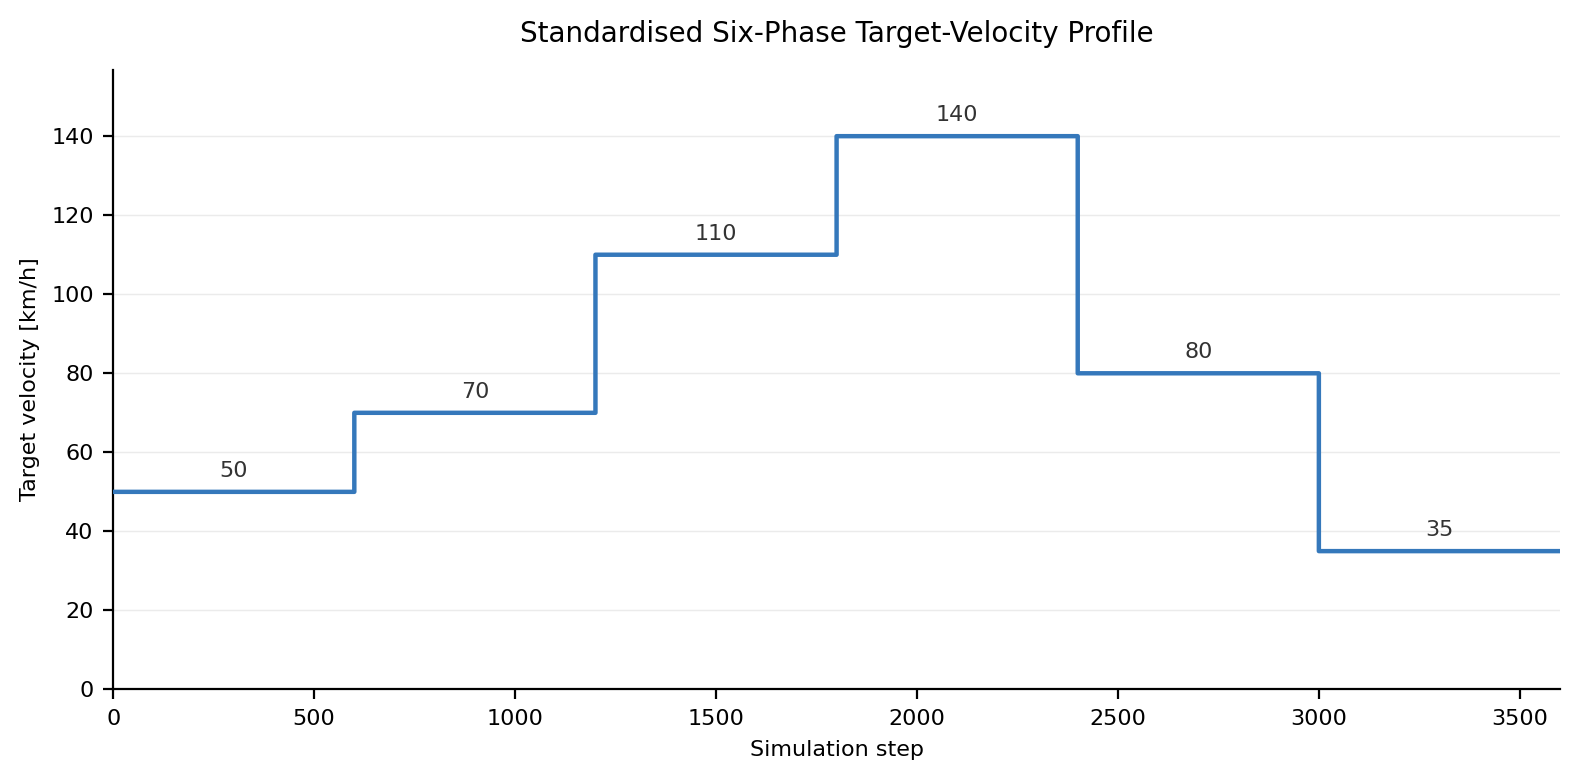
\includegraphics[width=\linewidth,height=0.42\textheight,keepaspectratio]{eval_target_profile.png}
    \end{column}
  \end{columns}
\end{frame}

%==============================================================================
\section{Phase 1 -- Feasibility \& the Twist}
%==============================================================================

% --- 9. PHASE 1 RESULT  (1:00) ------------------------------------------------
\begin{frame}{Phase 1: everyone learns to drive}
  All three algorithms track the speed cycle well -- \keyword{feasibility proven}.
  \vspace{0.6em}
  \begin{table}\centering\small
    \begin{tabular}{lccc}
      \toprule
      Metric (eval cycle) & PPO & TD3 & SAC \\
      \midrule
      RMSE speed [km/h] & $4.19\pm0.98$ & $3.81\pm0.29$ & $\mathbf{3.45\pm0.43}$ \\
      Cumulative \NOx{} [g] & $48.3$ & $95.4$ & $63.8$ \\
      $\Delta$SOC & $+0.25$ & $+0.15$ & $+0.19$ \\
      \bottomrule
    \end{tabular}
  \end{table}
  \vspace{0.4em}
  All under 5\,km/h RMSE. \alert{But the \NOx{} and battery numbers hide something...}
\end{frame}

% --- 10. THE TWIST  (2:30)  *** A-CLIMAX #1 *** -------------------------------
\begin{frame}{The twist: equal tracking, very different behaviour}
  \begin{columns}[T]
    \begin{column}{0.5\textwidth}
      \alert{Looking clean is easy if you cheat.}
      \begin{itemize}
        \item Same speed reward $\to$ wildly different powertrain use.
        \item The ``cleanest'' Phase 1 seed (SAC, \keyword{2.6\,g \NOx{}}) got there by \alert{draining the battery} ($\Delta$SOC $=-0.64$).
        \item Only \keyword{1 of 30} seeds was charge-sustaining -- and it emitted \keyword{60.9\,g \NOx{}}.
      \end{itemize}
      \vspace{0.4em}
      \begin{block}{Lesson}
        Low \NOx{} is \keyword{meaningless} without a \keyword{charge-sustaining constraint}. $\Rightarrow$ motivates Phase 2.
      \end{block}
    \end{column}
    \begin{column}{0.5\textwidth}
      \centering
      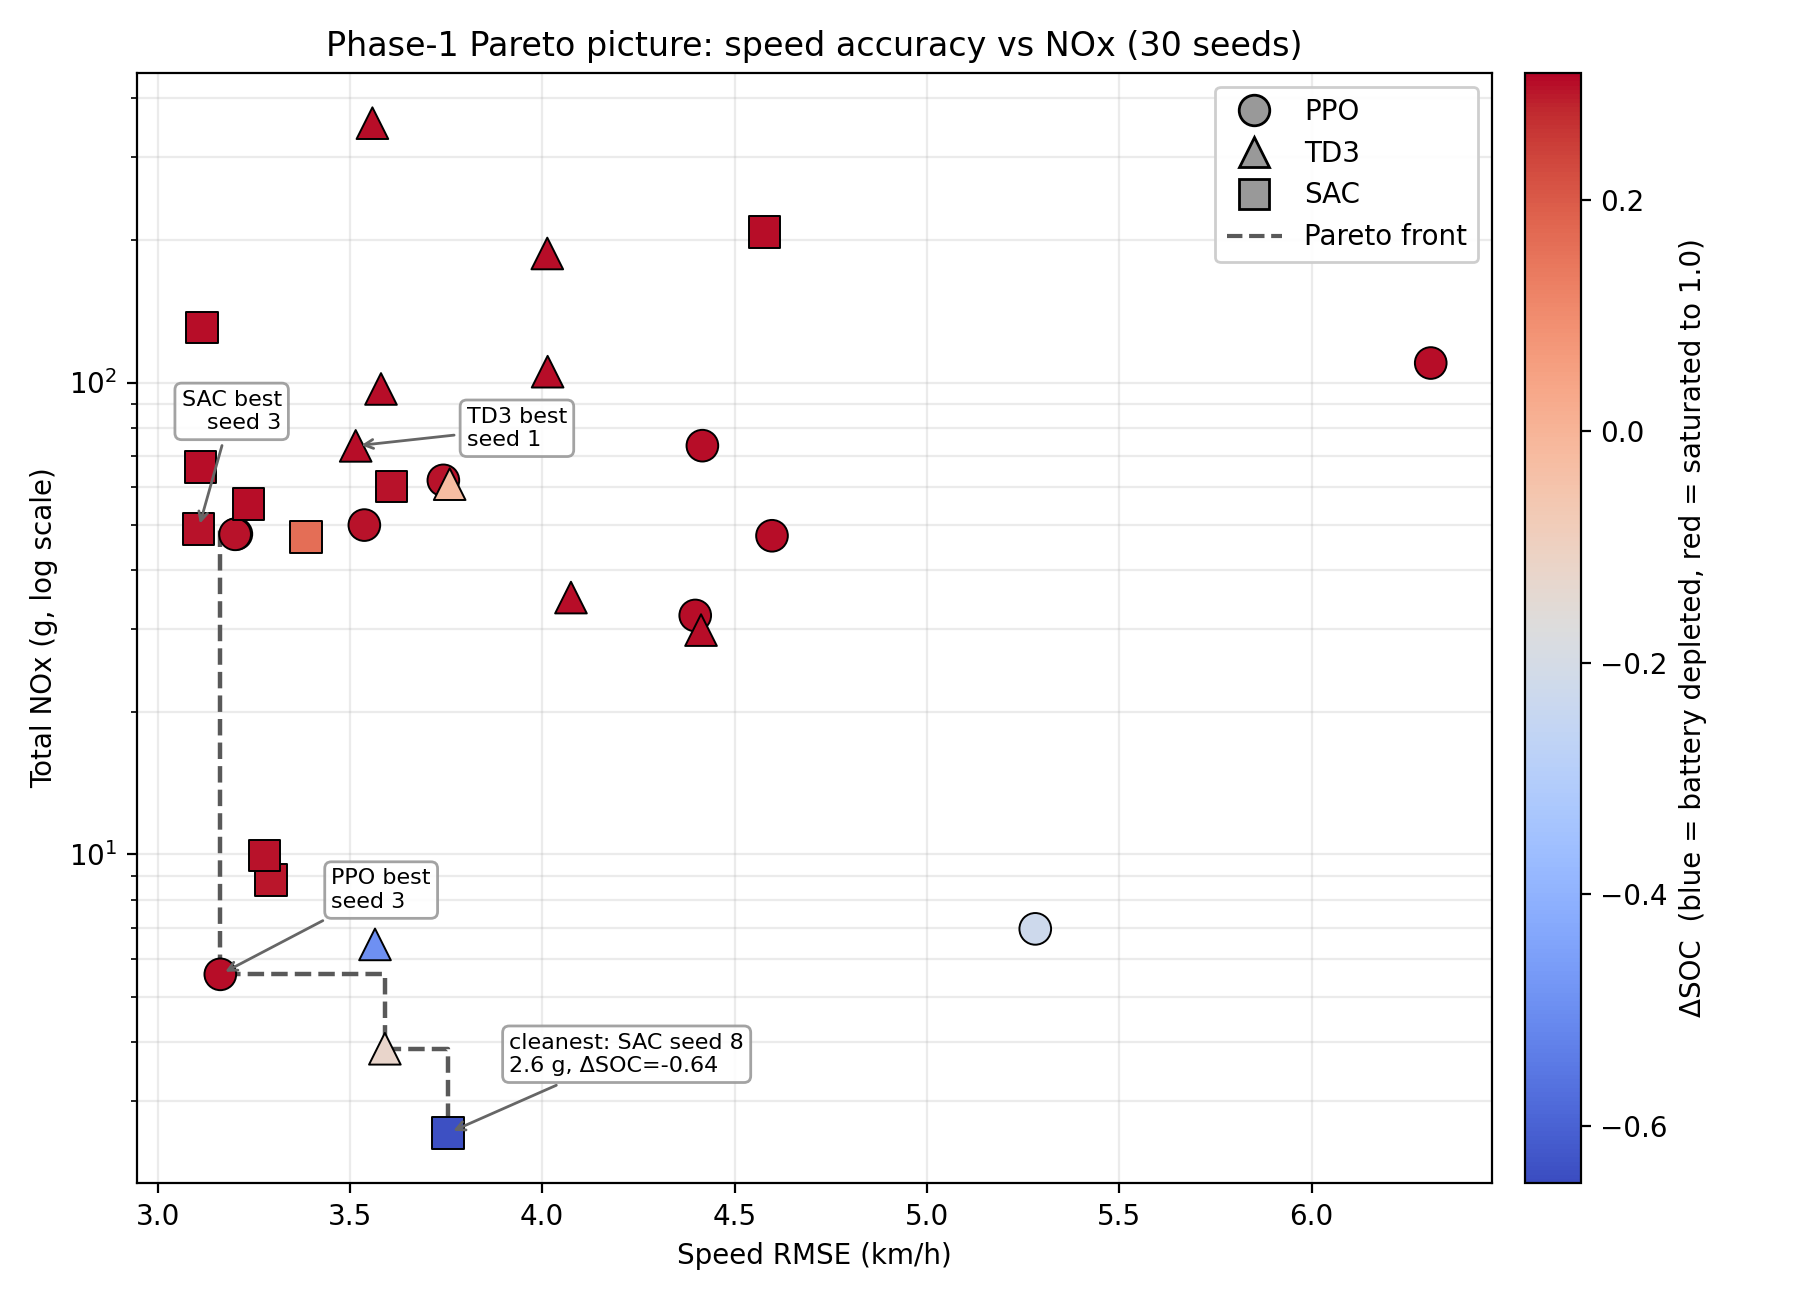
\includegraphics[width=\linewidth,height=0.80\textheight,keepaspectratio]{analysis_plots/pareto_front.png}
      \par\tiny Colour = $\Delta$SOC. Low-\NOx{} front = battery-depleters.
    \end{column}
  \end{columns}
\end{frame}

%==============================================================================
\section{Phase 2 -- Multi-Objective Control}
%==============================================================================

% --- 11. PHASE 2 RESULT  (2:00) -----------------------------------------------
\begin{frame}{Phase 2: fix it with \NOx{} + SOC penalties}
  Fine-tune from Phase 1; activate \NOx{} and SOC reward terms.
  \begin{table}\centering\small
    \begin{tabular}{lccc}
      \toprule
      Metric (P1 $\to$ P2) & PPO & TD3 (8/10) & SAC \\
      \midrule
      RMSE [km/h] & $4.19\to\mathbf{3.13}$ & $3.81\to3.96$ & $3.45\to3.33$ \\
      \NOx{} [g] & $48.3\to\mathbf{4.9}$ & $95.4\to8.7$ & $63.8\to\mathbf{4.5}$ \\
      Fuel [g] & $79.6\to52.8$ & $122.6\to79.5$ & $113.5\to64.0$ \\
      $|\Delta$SOC$|$ & $0.25\to\mathbf{0.03}$ & $0.15\to0.07$ & $0.19\to\mathbf{0.01}$ \\
      \bottomrule
    \end{tabular}
  \end{table}
  \vspace{0.3em}
  \keyword{\NOx{} down $\sim$10$\times$, SOC drift down $\sim$10$\times$, tracking kept (even improved).}
  \begin{center}
    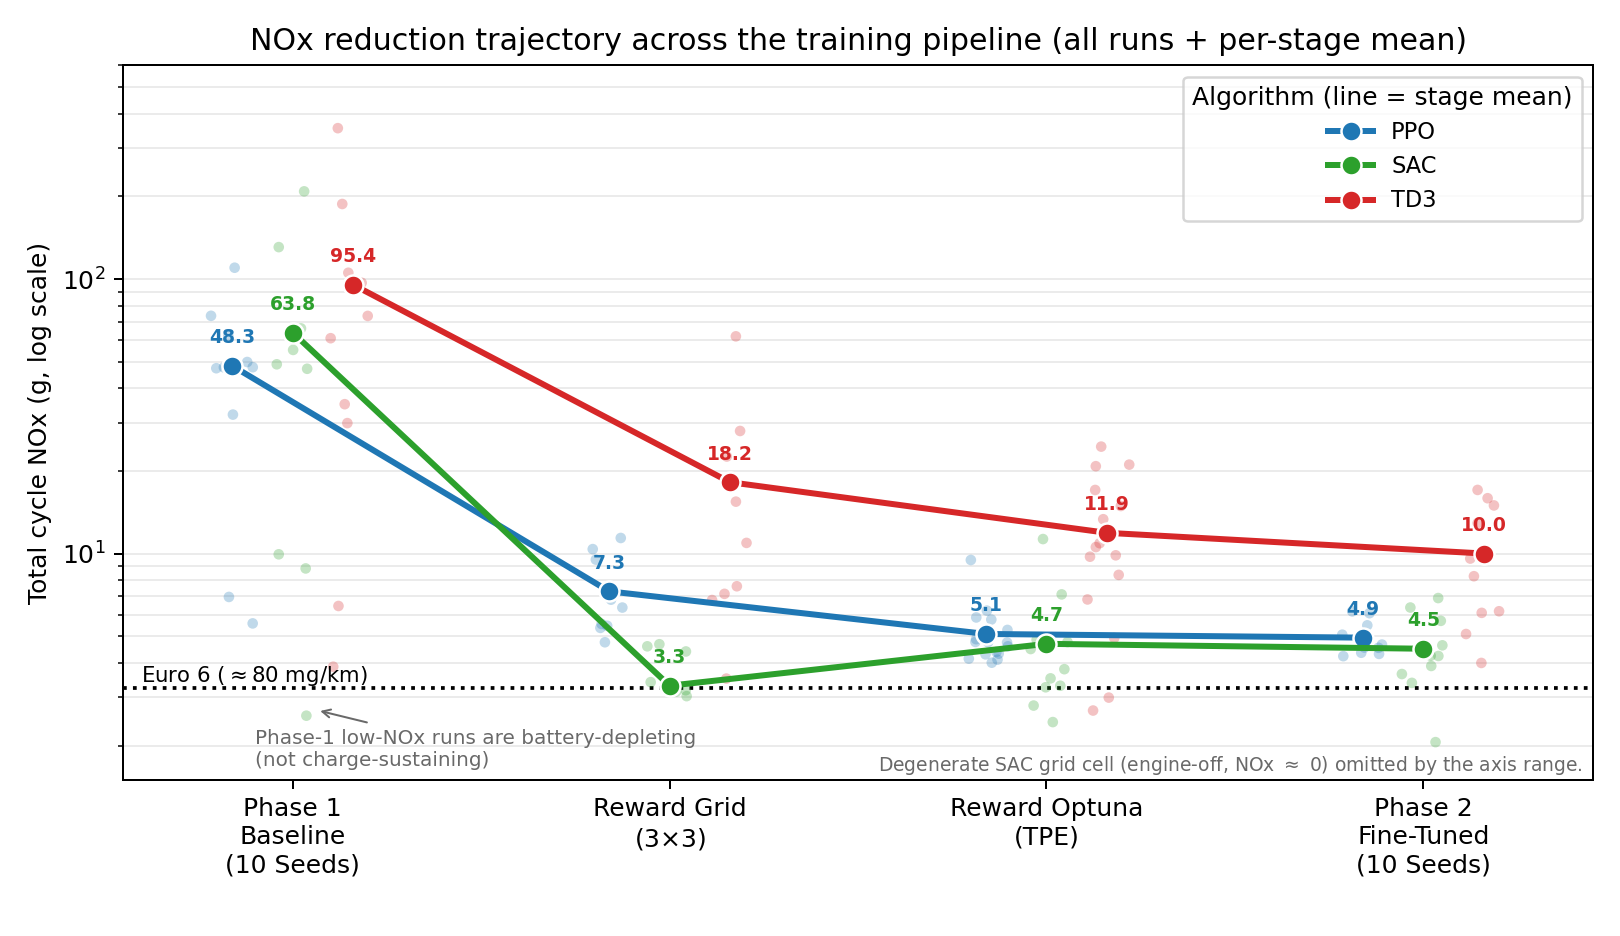
\includegraphics[width=0.52\textwidth,height=0.34\textheight,keepaspectratio]{nox_pipeline_swarm_traj.png}
  \end{center}
\end{frame}

% --- 12. MECHANISM  (1:30) ----------------------------------------------------
\begin{frame}{Why it works -- not a black box}
  \begin{columns}[T]
    \begin{column}{0.42\textwidth}
      \begin{itemize}
        \item \NOx{} rises \keyword{monotonically} with engine torque ($r=0.84$).
        \item Phase 2 shifts the engine to \keyword{lower load} $\to$ lower \NOx{}.
        \item Fuel drops \emph{too} -- but only because Phase 1 was \keyword{overcharging} the battery with wasteful high-load running.
      \end{itemize}
      \footnotesize\alert{Not a general \NOx{}--fuel synergy} -- it's removing wasted work.
    \end{column}
    \begin{column}{0.58\textwidth}
      \centering
      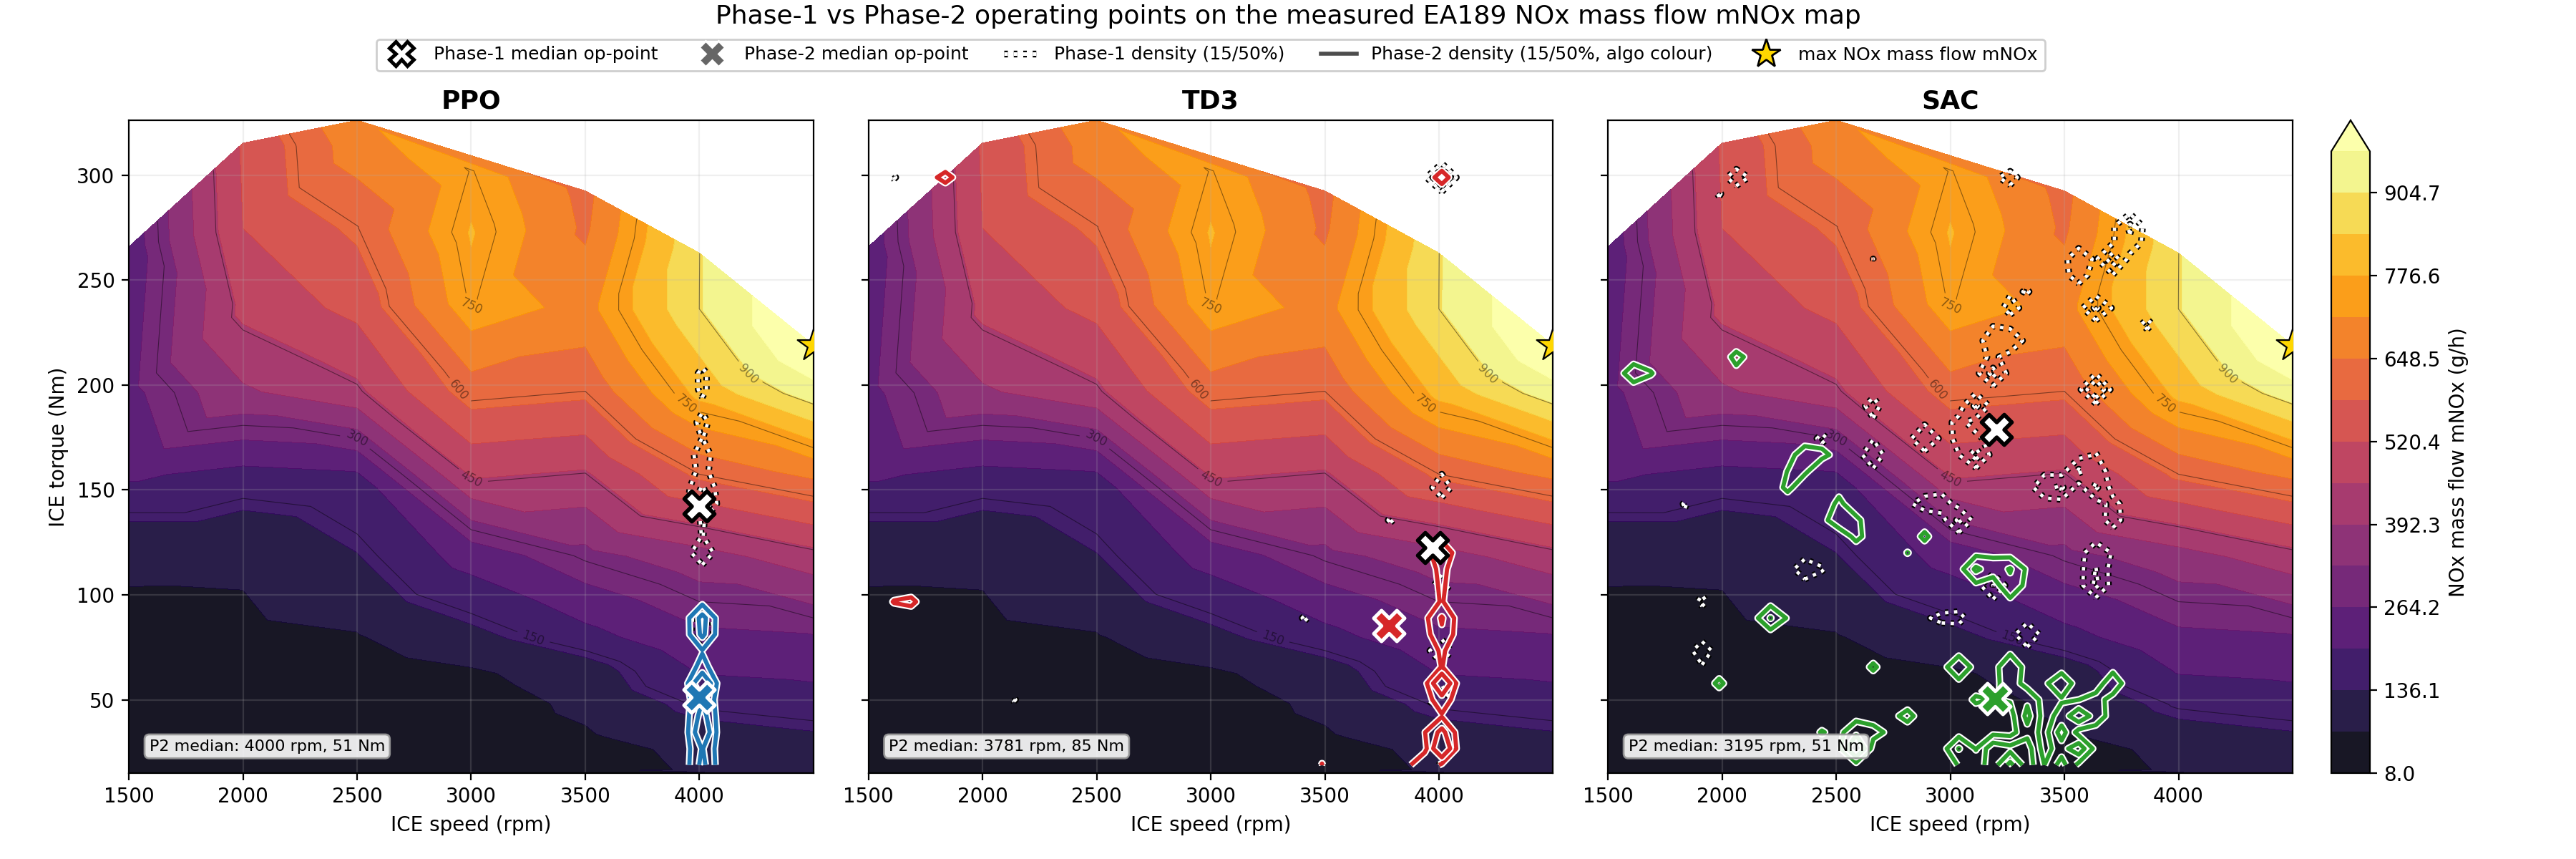
\includegraphics[width=\linewidth,height=0.52\textheight,keepaspectratio]{analysis_plots/phase2/engine_map_nox_overlay.png}
      \par\tiny Operating points move from bright (high-\NOx{}) into dark (low-\NOx{}) regions.
    \end{column}
  \end{columns}
\end{frame}

% --- 13. ALGORITHM VERDICT  (1:00) --------------------------------------------
\begin{frame}{Algorithm verdict}
  \begin{columns}[T]
    \begin{column}{0.5\textwidth}
      \begin{itemize}
        \item \keyword{PPO} -- most \keyword{robust}: tiny seed-to-seed variance, best tracking transfer.
        \item \keyword{SAC} -- \keyword{cleanest}: lowest \NOx{}, best single candidate.
        \item \honest{TD3 -- excluded}: unstable, 20\,\% of seeds fail to converge.
      \end{itemize}
    \end{column}
    \begin{column}{0.5\textwidth}
      \centering
      
\includegraphics[width=\linewidth,height=0.62\textheight,keepaspectratio]{plots/phase2/training_progress_comparison.png}
      \par\tiny TD3 (red) never stabilises; PPO/SAC converge cleanly.
    \end{column}
  \end{columns}
\end{frame}

%==============================================================================
\section{Generalisation: WLTC}
%==============================================================================

% --- 14. WLTC HONEST  (1:30)  *** LEAD WITH HONESTY *** -----------------------
\begin{frame}{Generalisation test: zero-shot on the real WLTC cycle}
  WLTC = standardised real-world driving cycle. Agents \keyword{never trained on it}.
  \vspace{0.5em}
  \begin{block}{The honest population-level result}
    Averaged over 10 seeds, the RL agents \alert{lose} to the rule-based controller:
    \begin{itemize}
      \item burn \alert{1.6--2.2$\times$ more fuel}, emit \alert{$\sim$17\,\% more \NOx{}}
      \item \keyword{but} track the target more tightly (RMSE 0.8--1.6 vs 2.3\,km/h)
    \end{itemize}
  \end{block}
  \footnotesize Reporting this loss is deliberate: fuel was \emph{never} in the reward -- a known blind spot.
  \begin{center}
    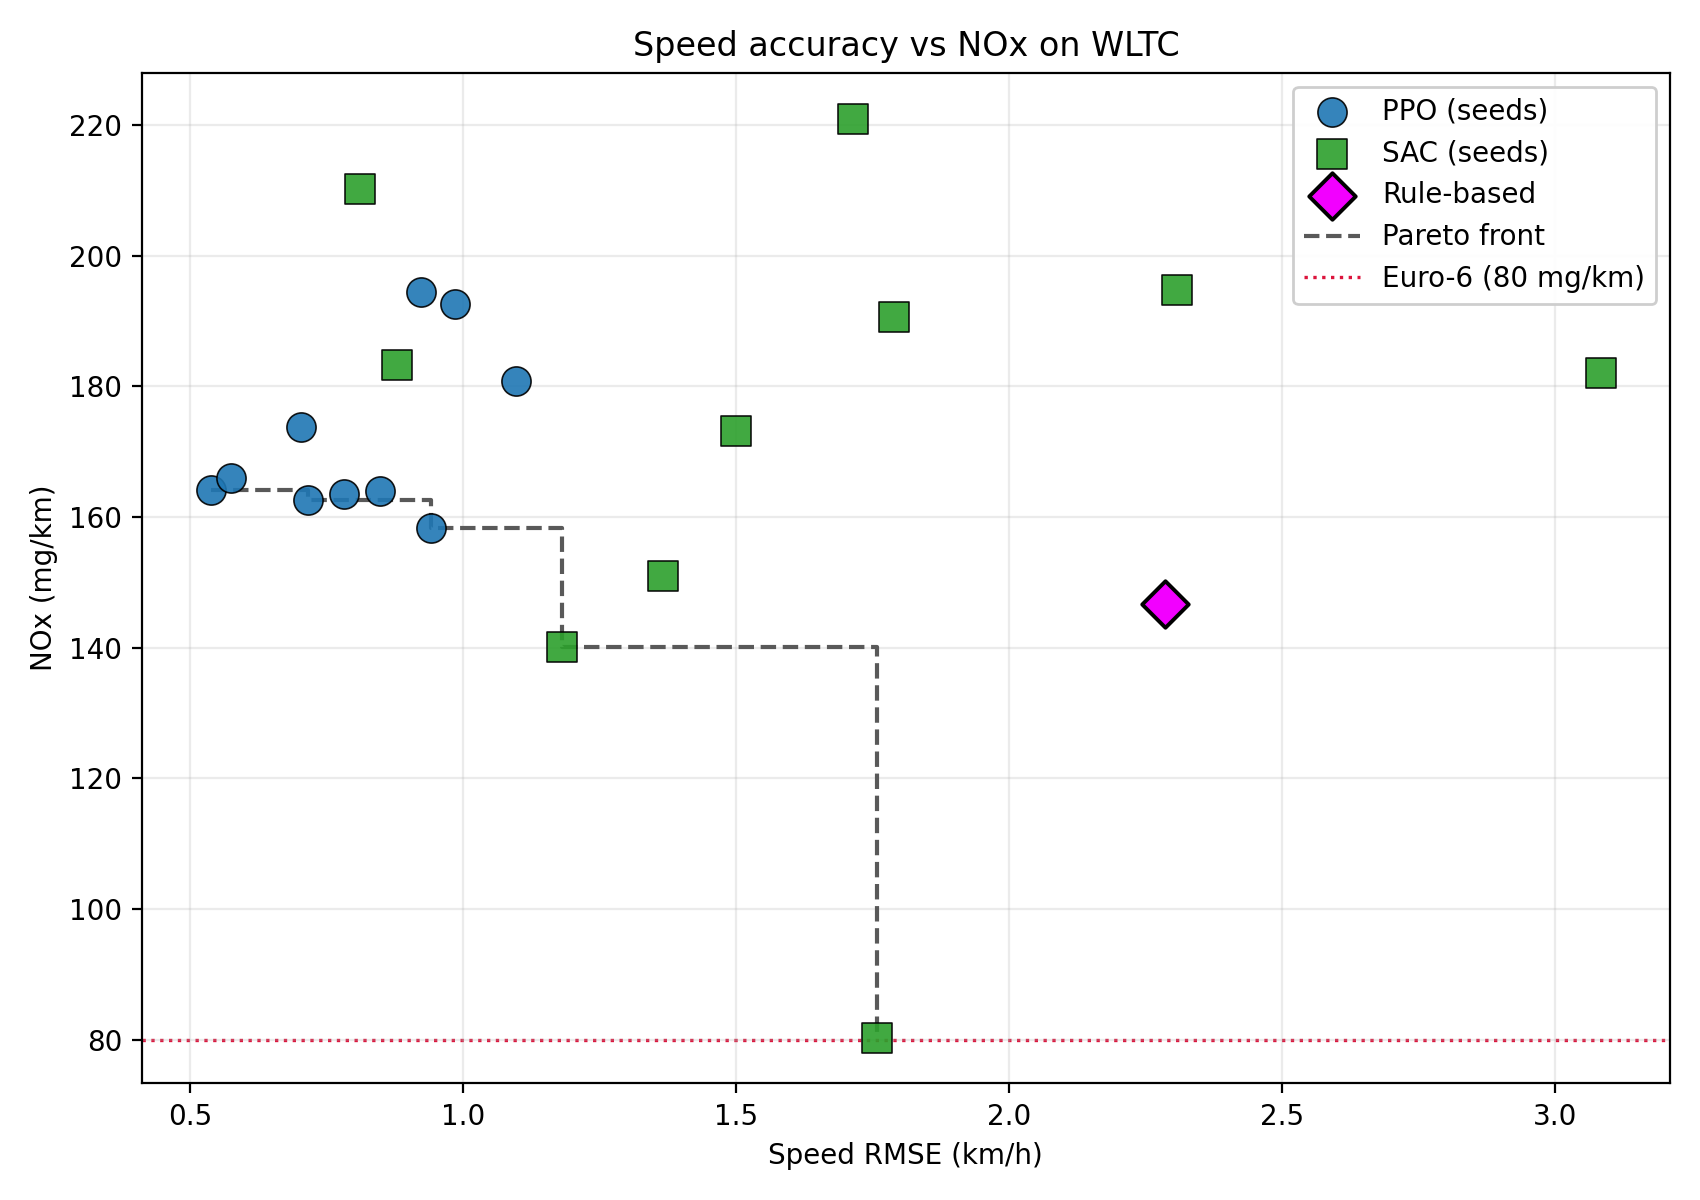
\includegraphics[width=0.48\textwidth,height=0.34\textheight,keepaspectratio]{plots/wltc_comparison/pareto_wltc.png}
  \end{center}
\end{frame}

% --- 15. WLTC BEST SEED  (1:30)  *** A-CLIMAX #2 *** --------------------------
\begin{frame}{But the right unit is a single controller, not an average}
  \alert{Averaging distinct policies describes no real controller.} Pick the best one.
  \begin{columns}[T]
    \begin{column}{0.52\textwidth}
      \begin{table}\centering\footnotesize
        \begin{tabular}{lcccc}
          \toprule
          & \NOx{} & Fuel & RMSE & $\Delta$SOC \\
          & mg/km & g & km/h & \\
          \midrule
          \keyword{SAC seed 7} & \keyword{80} & 1730 & 1.76 & $+0.01$ \\
          Rule-based & 147 & 1376 & 2.29 & $+0.00$ \\
          \bottomrule
        \end{tabular}
      \end{table}
      \vspace{0.4em}
      \keyword{SAC seed 7 hits Euro 6 (80 vs 147\,mg/km)}, tracks better, stays charge-neutral.
      \par\footnotesize Cost: $+26\,\%$ fuel, achieved by switching the engine off 57\,\% of the cycle.
    \end{column}
    \begin{column}{0.48\textwidth}
      \centering
      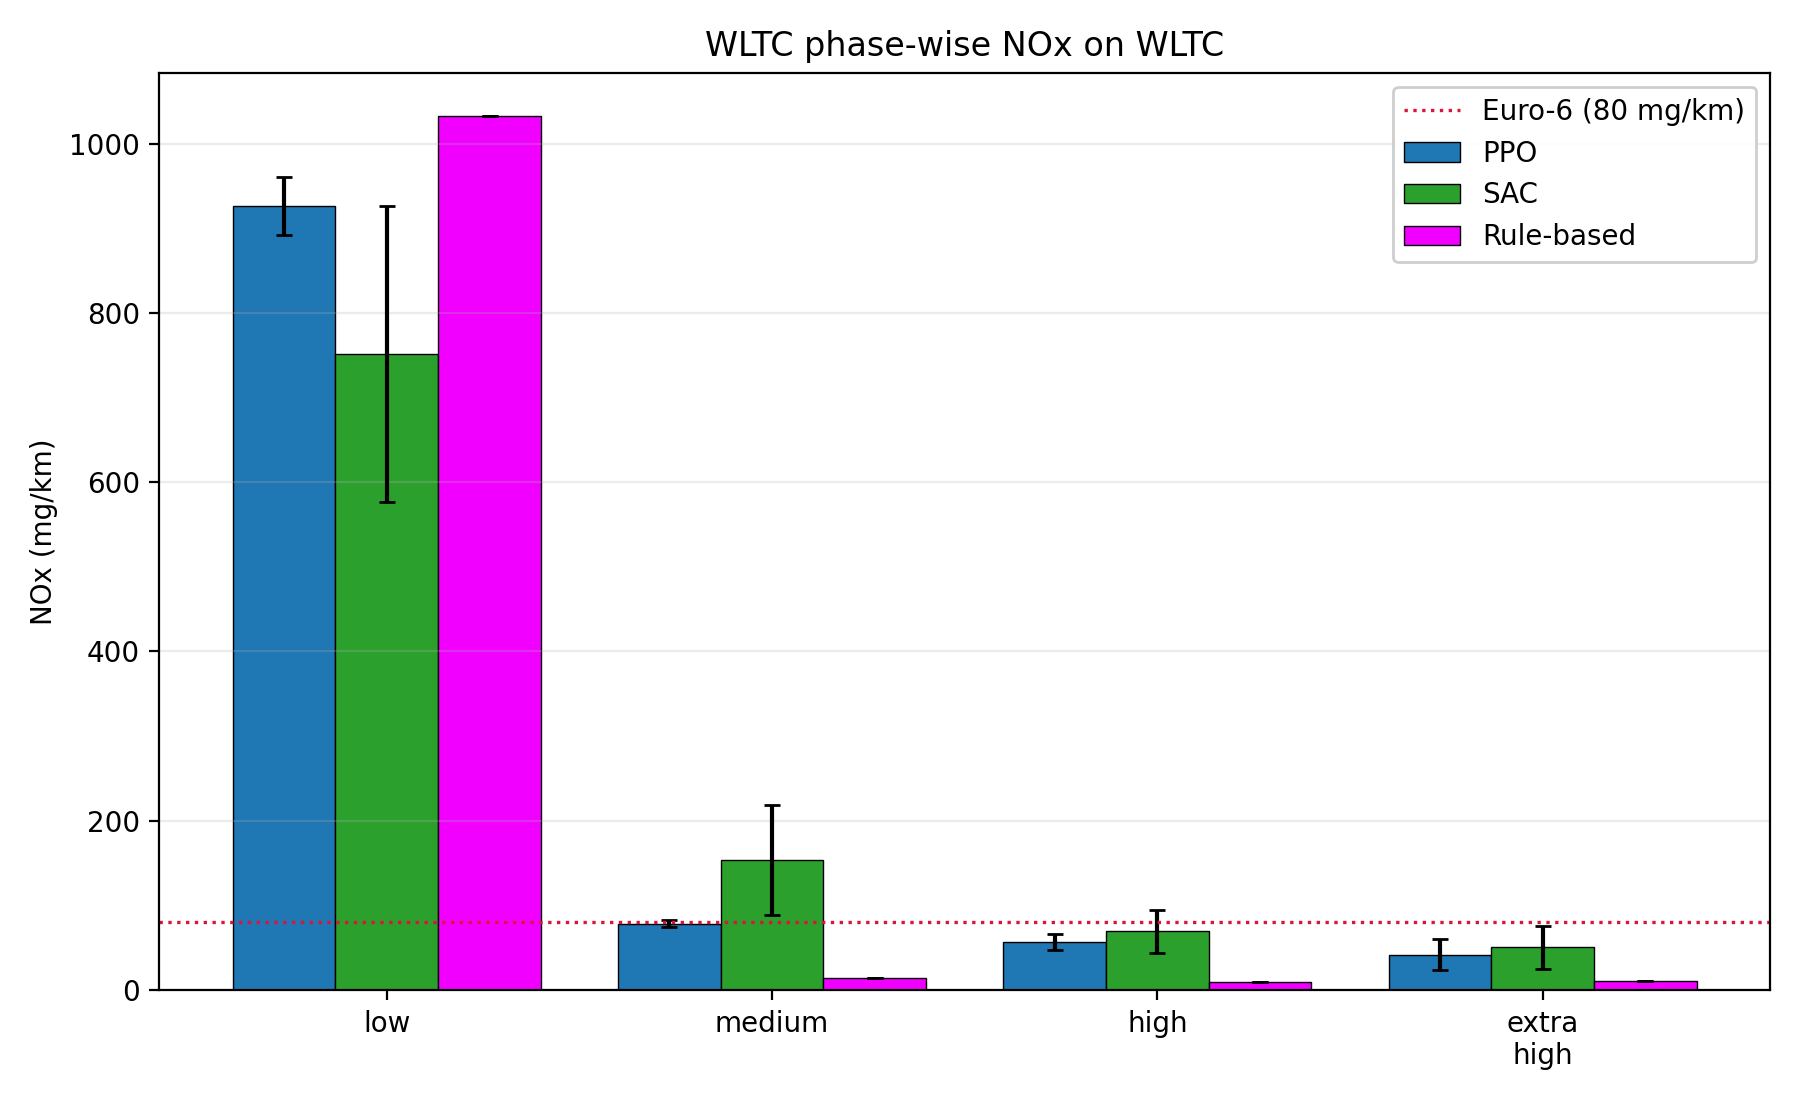
\includegraphics[width=\linewidth,height=0.66\textheight,keepaspectratio]{plots/wltc_comparison/phase_nox_wltc.png}
    \end{column}
  \end{columns}
\end{frame}

%==============================================================================
\section{Conclusion}
%==============================================================================

% --- 16. LIMITATIONS AS MATURITY  (1:00) --------------------------------------
\begin{frame}{Honest limitations = scope, not weakness}
  \begin{itemize}
    \item \honest{Single pollutant.} Only \NOx{} optimised -- no fuel/CO\textsubscript{2} term. \emph{The} main gap.
    \item \honest{Surrogate only.} Validated against LSTM models, not a real engine -- sim-to-real open.
    \item \honest{Engine-specific.} Models tied to the EA189; the \emph{methodology} transfers, the models don't.
    \item \honest{Asymmetric baseline.} Rule-based = 1 run; RL = 10 seeds. Informative, not a strict superiority test.
  \end{itemize}
  \vspace{0.5em}
  \begin{center}
    \emph{This is a proof of concept -- feasibility shown, deployment not claimed.}
  \end{center}
\end{frame}

% --- 17. CONCLUSION  (1:30) ---------------------------------------------------
\begin{frame}{Conclusion \& outlook}
  \begin{columns}[T]
    \begin{column}{0.55\textwidth}
      \textbf{Contributions}
      \begin{itemize}\footnotesize
        \item surrogate-based DRL control framework
        \item curriculum-inspired two-phase training
        \item comparative PPO / SAC / TD3 study
        \item zero-shot WLTC generalisation test
        \item design guidance for the LDCI2027 project
      \end{itemize}
    \end{column}
    \begin{column}{0.45\textwidth}
      \textbf{Headline}
      \begin{itemize}\footnotesize
        \item \NOx{} cut $\sim$10$\times$, charge-sustaining, tracking kept
        \item \keyword{SAC seed 7} reaches Euro 6 zero-shot $\to$ handed to LDCI2027
      \end{itemize}
      \textbf{Future work}
      \begin{itemize}\footnotesize
        \item add fuel / CO\textsubscript{2} reward term
        \item recurrent agents (true POMDP)
        \item hybrid rule-based + RL supervisor
      \end{itemize}
    \end{column}
  \end{columns}
\end{frame}

% --- THANK YOU ----------------------------------------------------------------
{\setbeamercolor{background canvas}{bg=tugreen}
\begin{frame}[plain]
  \centering
  \vfill
  {\color{white}\Huge \textbf{Thank you}}\\[1em]
  {\color{white}\large Questions?}
  \vfill
\end{frame}}

% --- BACKUP SLIDES (for Q&A) --------------------------------------------------
\appendix
\begin{frame}{Backup: full Phase 2 training curves}
  \centering
  
\includegraphics[width=0.7\textwidth,height=0.78\textheight,keepaspectratio]{plots/phase2/training_progress_comparison.png}
\end{frame}

\begin{frame}{Backup: \NOx{} rate vs engine torque ($r=0.84$)}
  \centering
  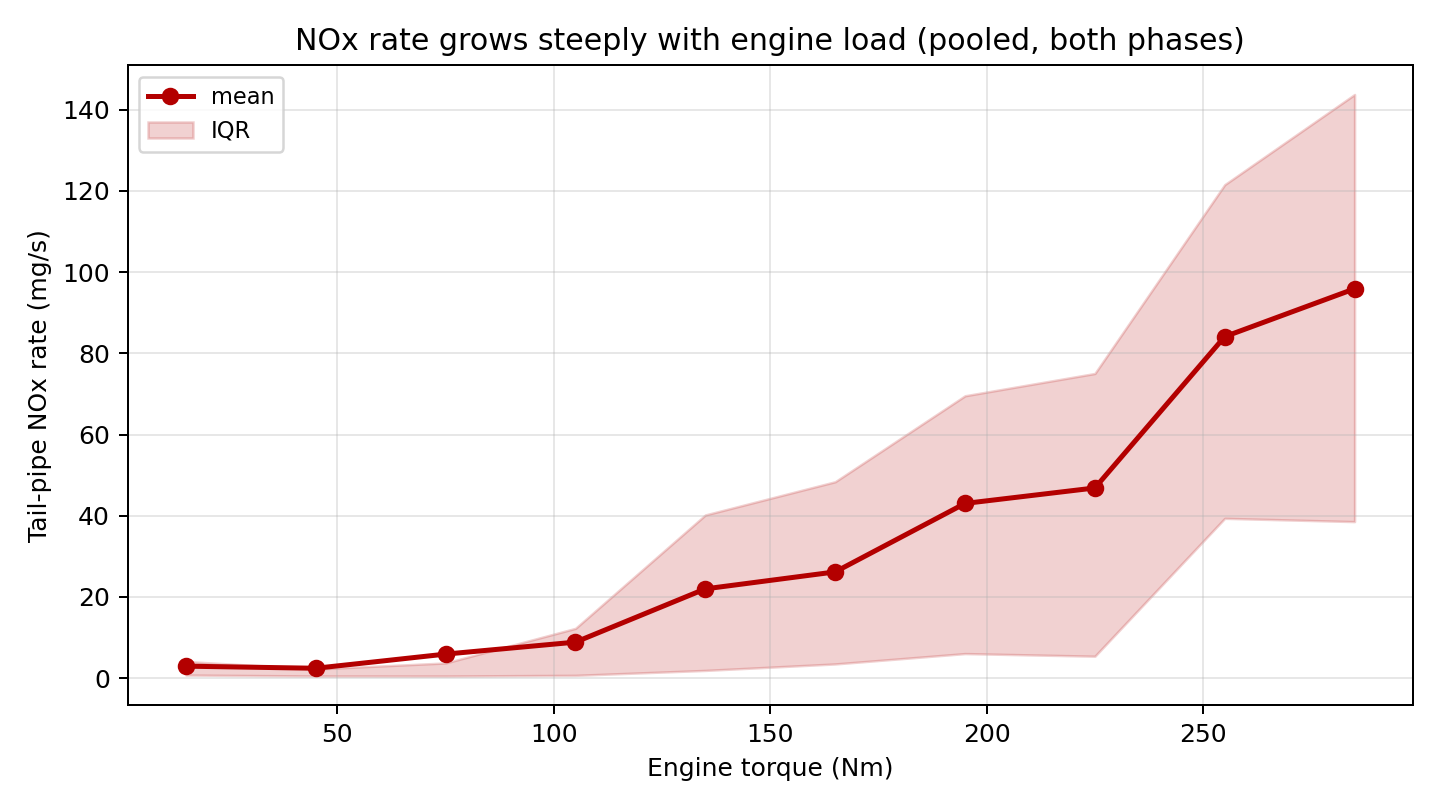
\includegraphics[width=0.62\textwidth,height=0.78\textheight,keepaspectratio]{analysis_plots/phase2/nox_rate_vs_torque.png}
\end{frame}

\begin{frame}{Backup: BSFC engine-map operating points (P1 vs P2)}
  \centering
  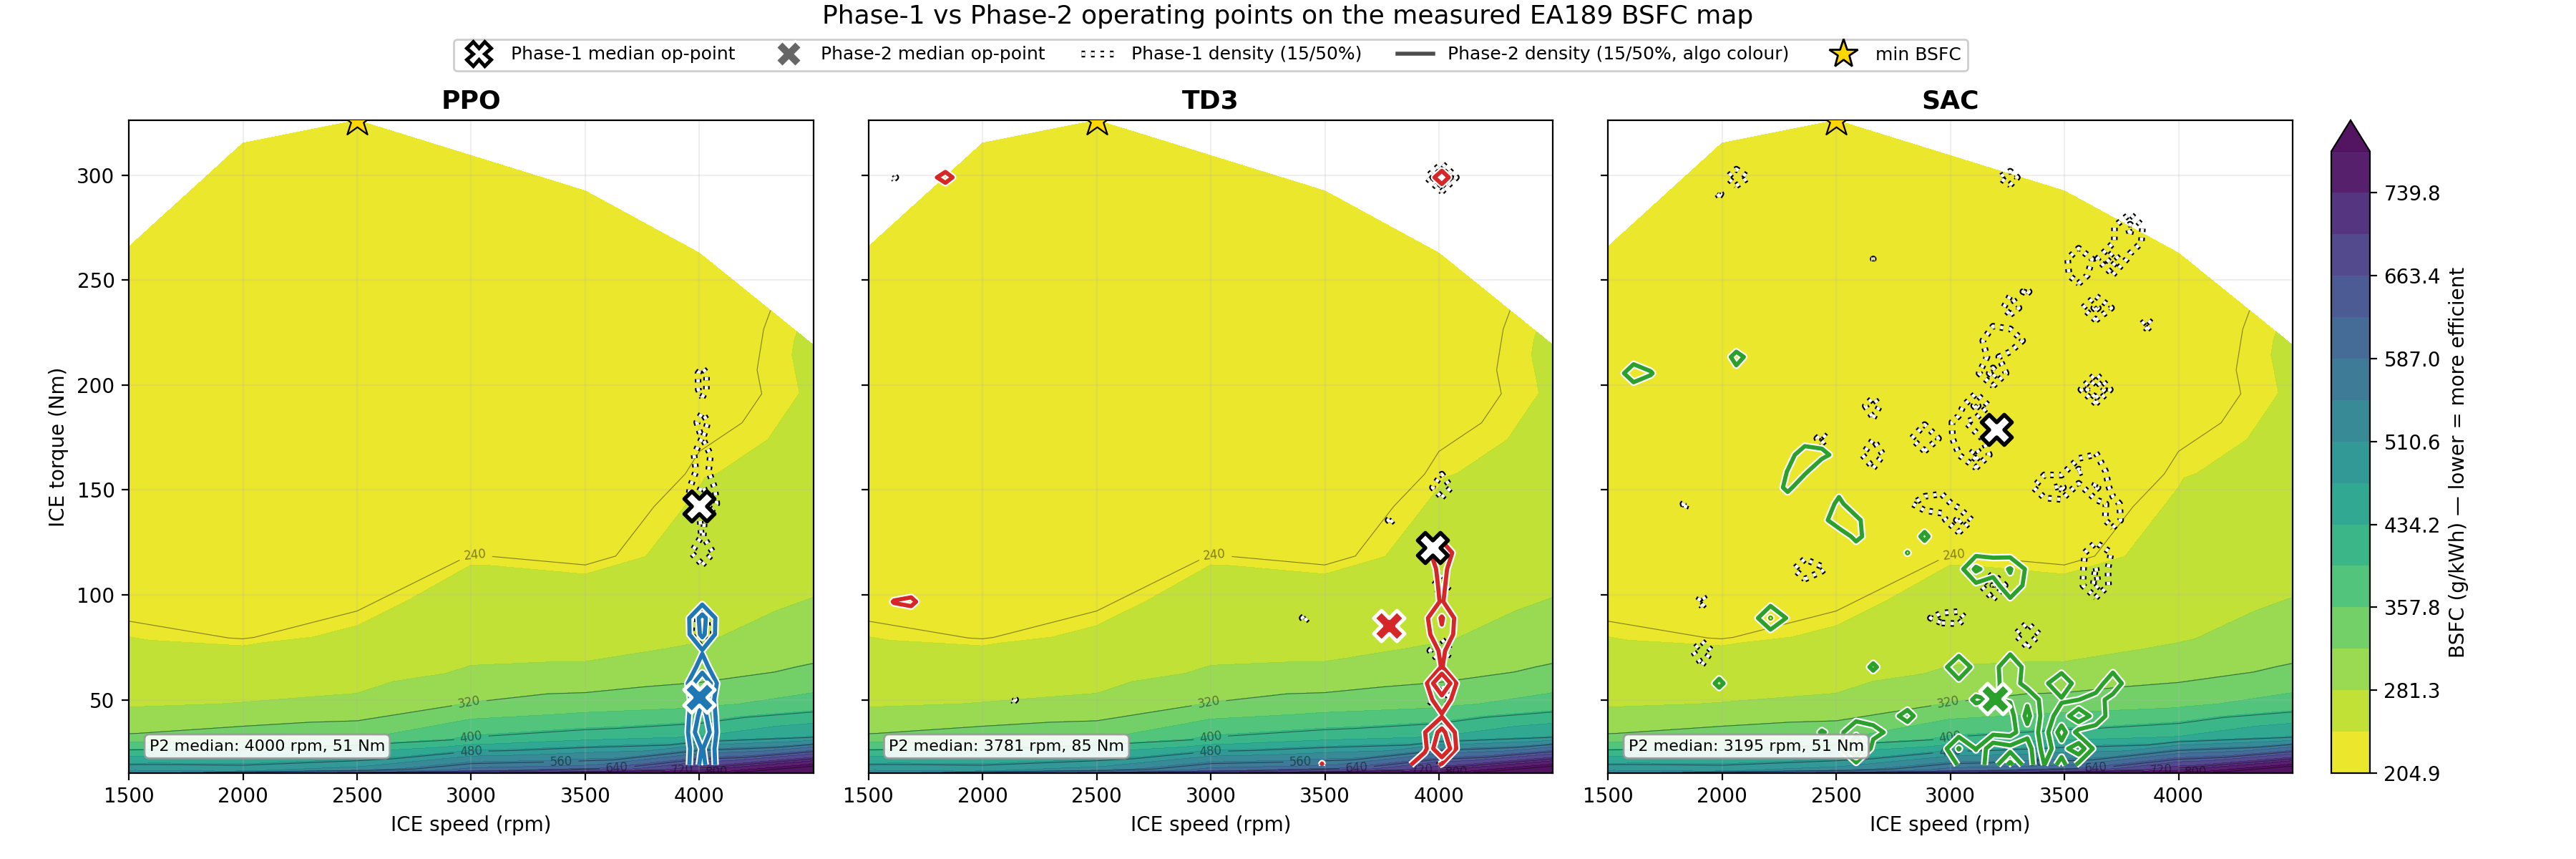
\includegraphics[width=\textwidth,height=0.78\textheight,keepaspectratio]{analysis_plots/phase2/engine_map_bsfc_overlay.png}
\end{frame}

\begin{frame}{Backup: SAC seed 7 on WLTC -- full trace}
  \centering
  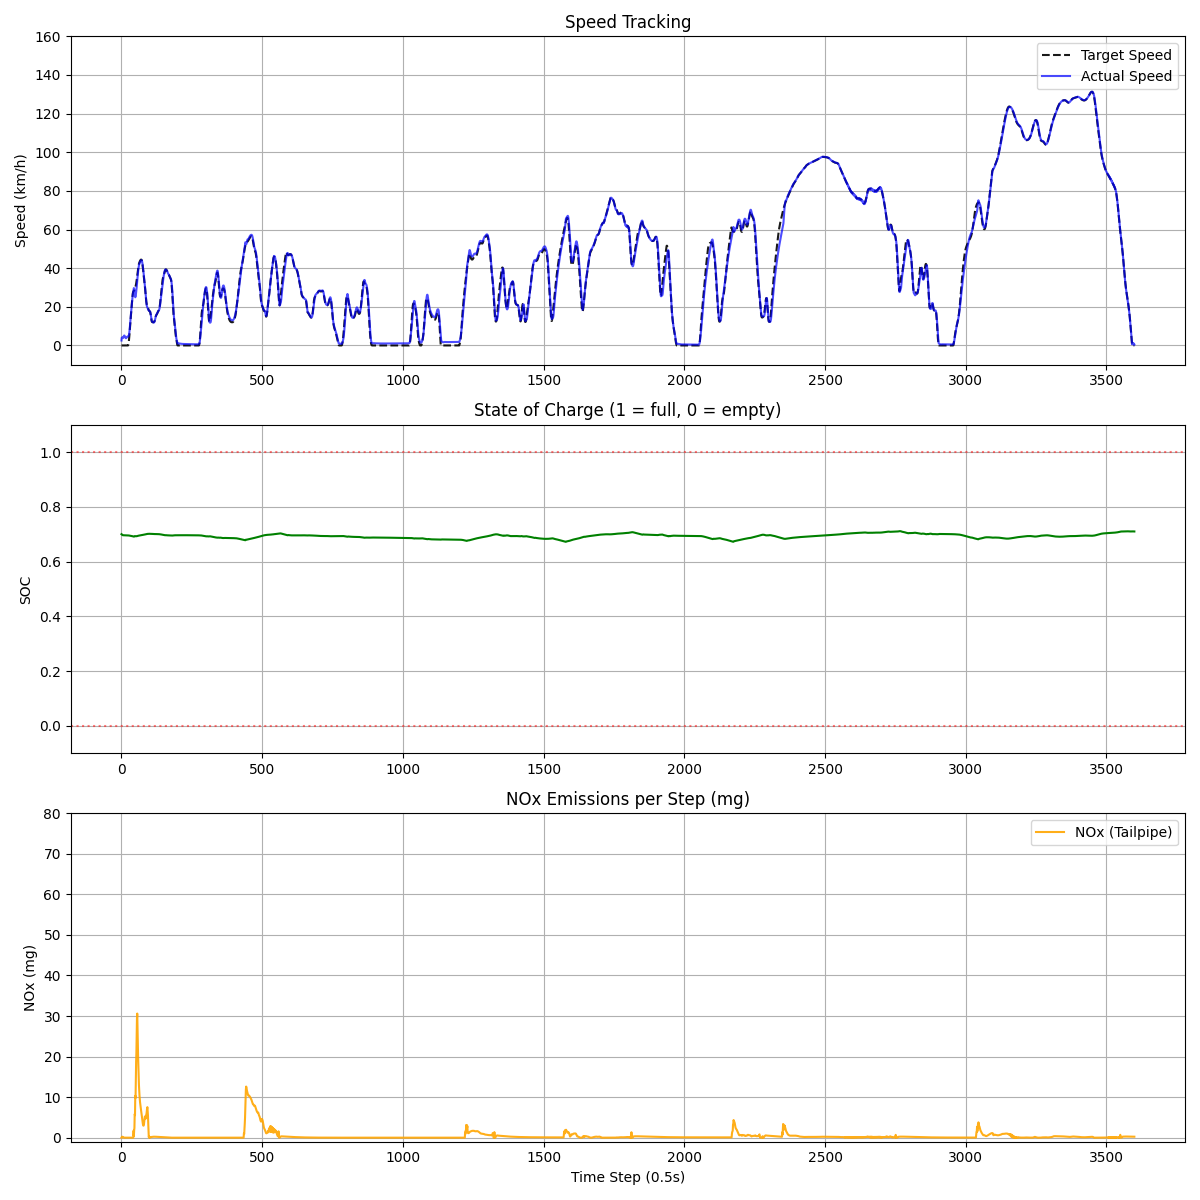
\includegraphics[width=0.6\textwidth,height=0.78\textheight,keepaspectratio]{plots/wltc_comparison/seed_7_wltc_evaluation_results.png}
\end{frame}

\begin{frame}{Backup: WLTC speed tracking (10-seed band)}
  \centering
  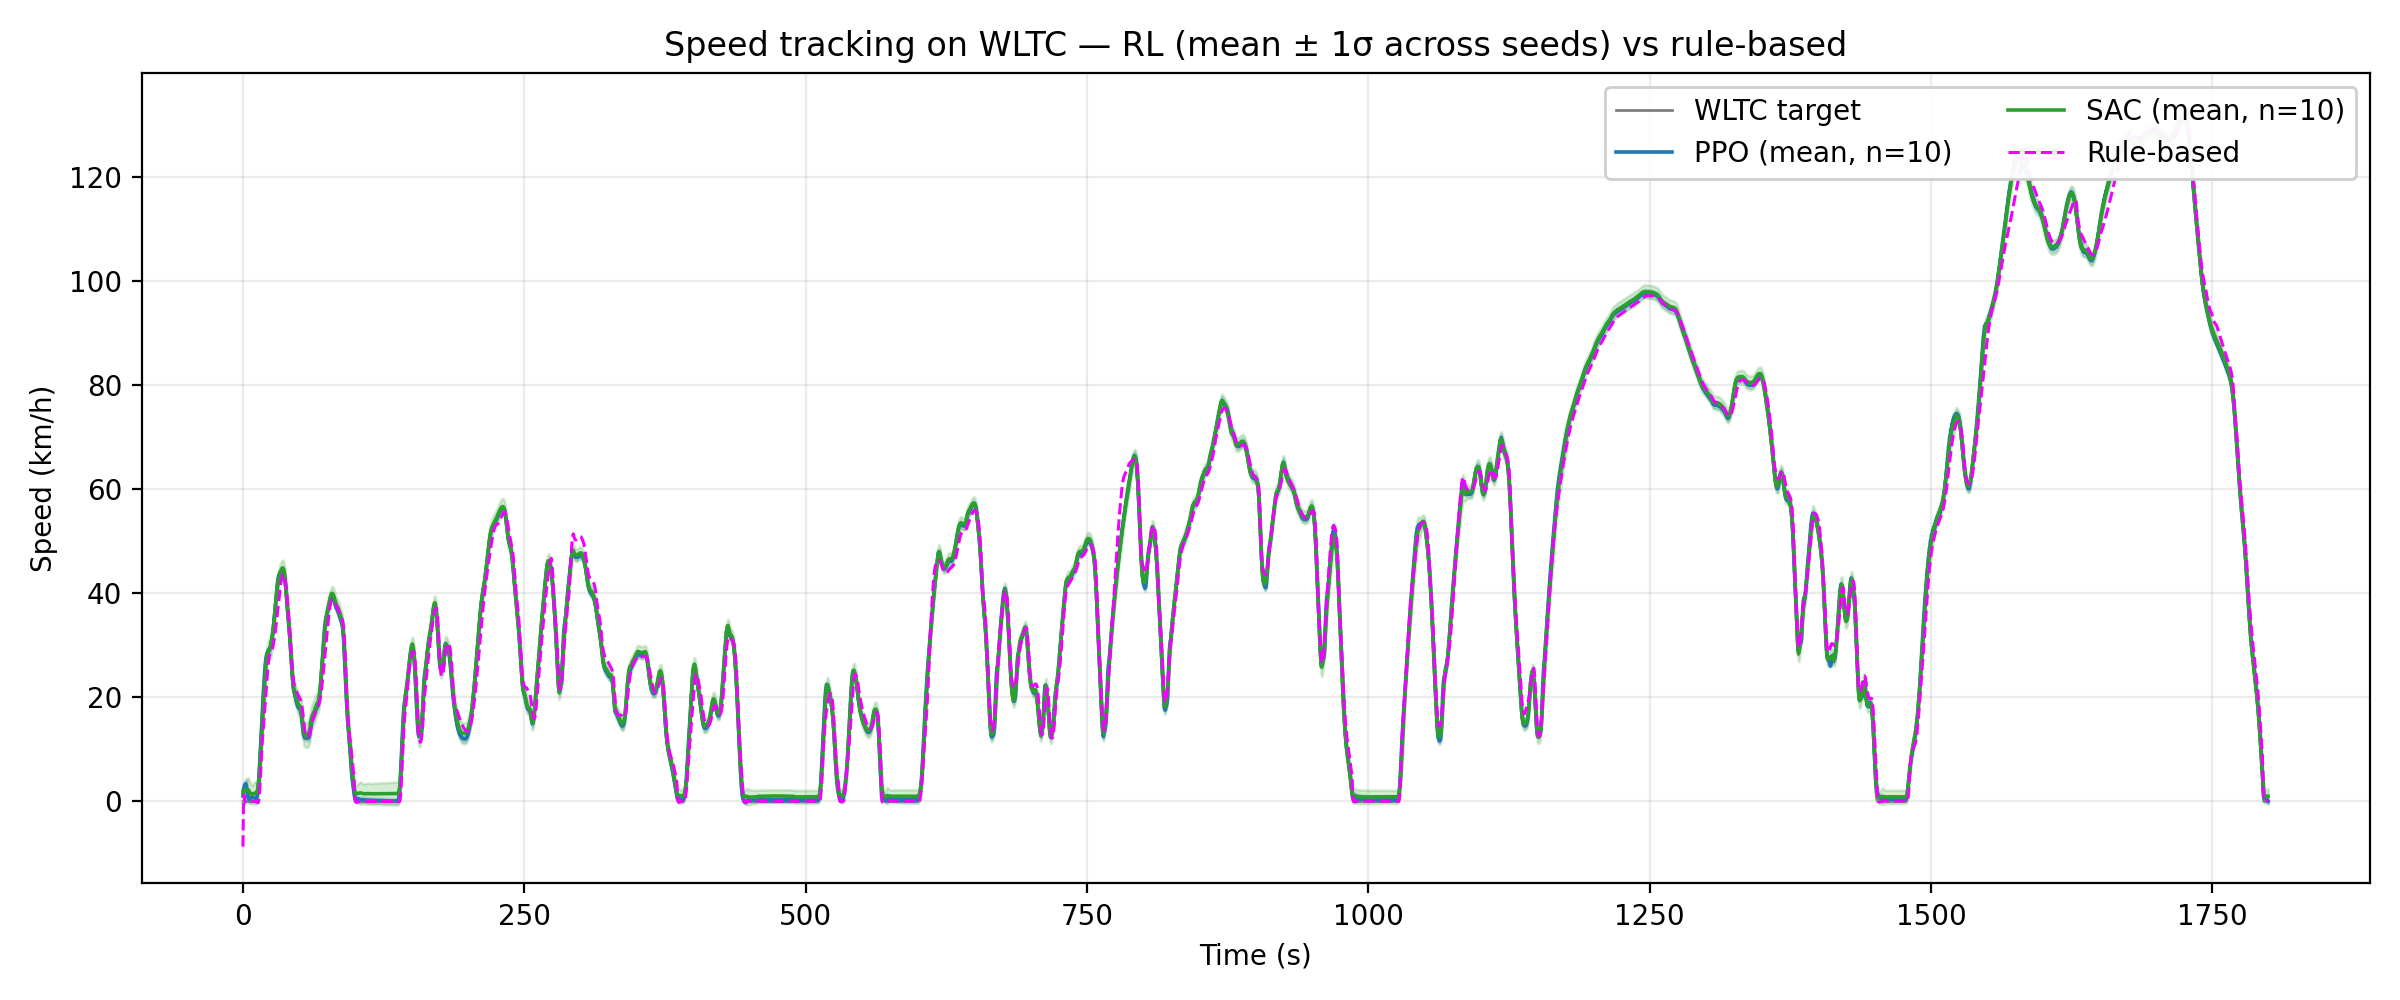
\includegraphics[width=0.85\textwidth,height=0.78\textheight,keepaspectratio]{plots/wltc_comparison/speed_tracking_wltc.png}
\end{frame}

\end{document}
